\section{Нейтронно-физический расчет}

\subsection{Постановка задачи}
В рамках данного этапа работы будет выполнены следующие задачи:
\begin{enumerate}
    \item Ячеечный расчет для определения характеристик ТВС в приближении бесконечной решетки
        \subitem Расчет ячеек без выгорания
        \subitem Построение модели полиячеек и их расчет без выгорания
        \subitem Расчет длительности цикла и выгорания при частичных перегрузках
    \item Расчет энерговыделения и коэффициента неравномерности активной зоны в приближении гомогенизированных ячеек
\end{enumerate}

\subsection{Описание инструмента ячеечного расчета}
Для расчета свойств ТВС использовались возможности программного комплекса GETERA-93 %\cite{белоусов2002использование}. 
Программа представляет собой инструмент для расчета нейтронно-физических характеристик активной зоны методом вероятностей первых столкновений, предоставляющий одномерный расчет активных зон сложной геометрии благодаря полиячеечным расчетам.

Данная программа разрабатывалась для группового расчета полей нейтронов на основе метода вероятностей первых столкновений (ВПС) полей нейтронов в ячейках реакторов, содержащих элементы с различной геометрией.
\subsection{Модель ячейки}
Для проведения расчетов определим исходные характеристики ТВС РУ-ВВЭР-1000 %\cite{ТвэлТерновых} 

\begin{table}[H]
	\caption{Исходные данные для ТВС проектируемого РУ ВВЭР-1000 }
	\begin{center}
        \begin{tabular}{|l|c|}
        \toprule
         Характеристика & Значение \\ 
         \midrule
          Форма ТВС & Шестигранная\\
         \hline
          Количество твэлов в ТВС & 317\\
         \hline
         Топливо & $\text{U}\text{O}_2$ \\
         \hline
         Обогащение топлива, \%& 4.7 \\
         \hline
         Плотность топлива, $\text{г}/\text{см}^3$ & 9.015 \\
         \hline
         Количество циклов перегрузки топлива & 3 \\
         \hline
         Состав оболочки & $99\% \text{Zr} + 1 \% \text{Nb}$ \\
         \hline
         Замедлитель & $\text{H}_2\text{O}$ \\
         \bottomrule
		\end{tabular}
		\label{tabular:neutron_in}
	\end{center}
\end{table}
\subsection{Расчет ячеек без выгорания}
Для расчета использовалась модель одномерной элементарной эквивалентной цилиндрической ячейки c радиусами $0.398, 0.455, 0.67$ мм. Геометрия элементарной ячейки представлена на рисунке \ref{pic:neutron_cell}

\begin{figure}[H]
	\begin{center}
		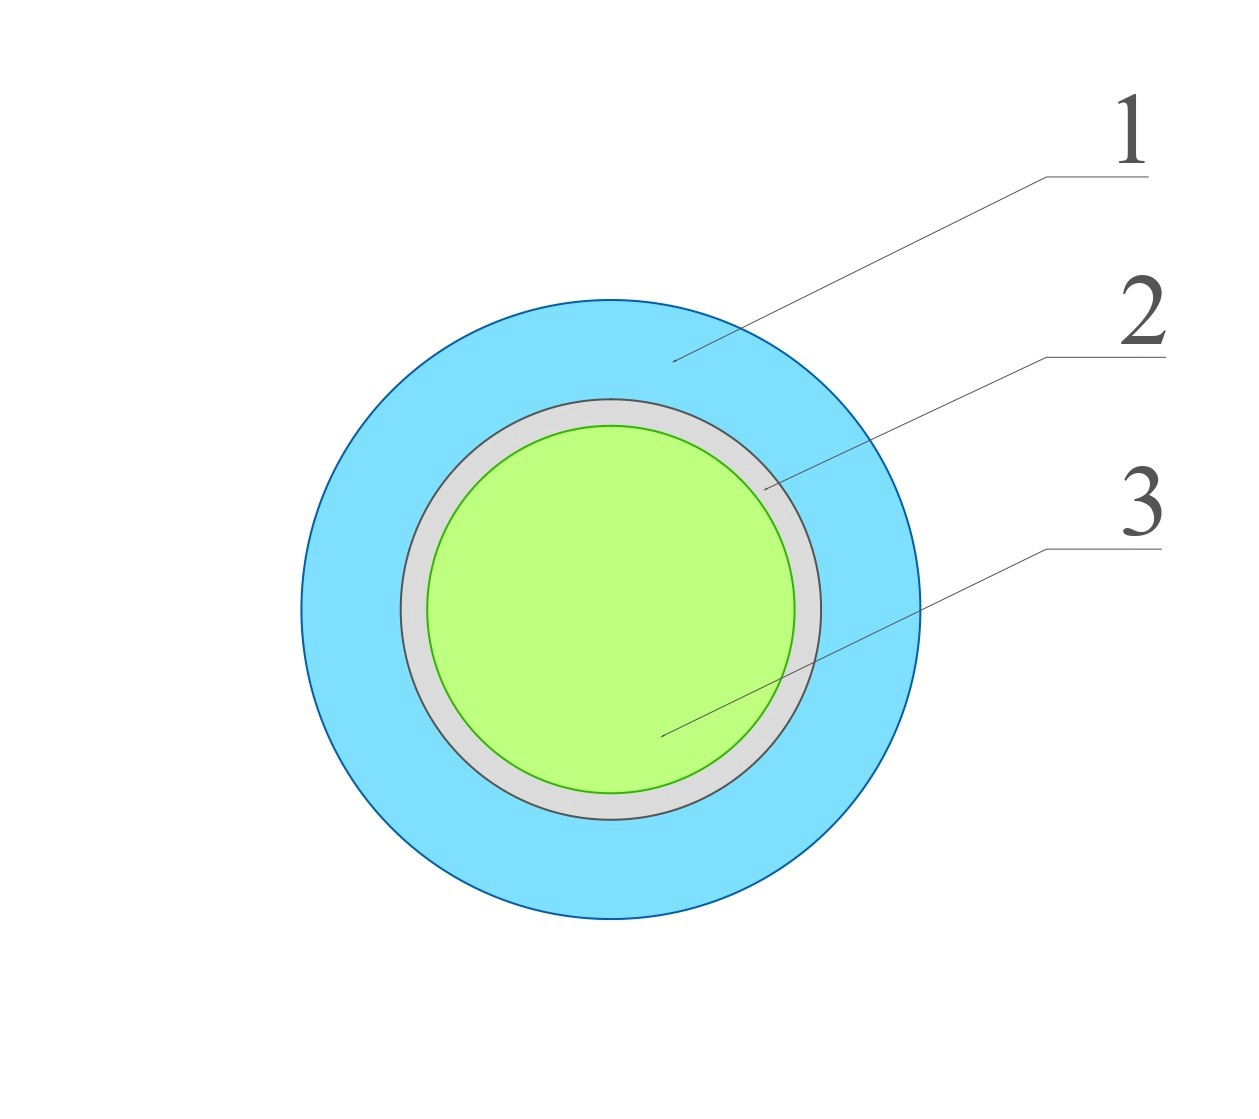
\includegraphics[scale=0.2]{cell.jpg}
		\caption{Геометрия элементарной топливной ячейки. 1 — замедлитель, 2 – оболочка, 3 – топливо}
		\label{pic:neutron_cell} % название для ссылок внутри кода
	\end{center}
\end{figure}
Рассчитаем необходимые концентрации элементов входящих в состав ячейки

\begin{table}[H]
	\caption{Концентрации элементов}
	\begin{center}
        \begin{tabular}{|l|c|}
        \toprule
         Элемент & Концентрация\\ 
         \midrule
          Топливо & \\
         \hline
          $\text{U}^{235}$ & $9.4518 \cdot 10^{-4}$\\
         \hline
          $\text{U}^{238}$ & $1.9165\cdot 10^{-2}$\\
         \hline
          $\text{O}$ & $4.02 \cdot 10^{-2}$\\
         \hline
         Оболочка & \\
         \hline
          $\text{Zr}$ & $4.25047 \cdot 10^{-2}$\\
         \hline
          $\text{Nb}$ & $5.55308\cdot 10^{-4}$\\
         \hline
         Замедлитель & \\
         \hline
         $\text{H}$ & $4.98456\cdot 10^{-2}$\\
         \hline
         $\text{O}$ & $2.49228\cdot 10^{-2}$\\
         \bottomrule
		\end{tabular}
		\label{tabular:neutron_conc}
	\end{center}
\end{table}
Используя входные данные зададим расчетную ячейку с указанными в \ref{tabular:neutron_conc} составами и радиусами.
Произведем расчет $K_{\infty}$ бесконечной решетки твс заданной модели с помощью команды \texttt{:FIER} заданной во входном файле расчета GETERA-93. Результрующее значение:
$$
K_{\infty} = 1.38
$$
\subsection{Расчет полиячеек без выгорания}
Перед дальнейшими расчетами выгорания необходимо усложнить модель активной зоны, представив ее бесконечной решеткой  полиячеек. Такой подход позволит учесть ячейки с различной степенью выгорания в активной зоне для дальнейшего расчета при использовании частичиных перегрузок. 

Разобьём ячейку на 3 фрагмента (в соответствии с заданным количество циклов выгорания), для которых предполагается применимым одномерное приближение. Связи между фрагментами зададим с помощью следующей матрицы перетечек записанной в переменную \texttt{ALOUT} расчетного файла:
$$
\begin{pmatrix}
0.0 & 0.5 & 0.5 \\ 
0.5 & 0.0 & 0.5 \\
0.5 & 0.5 & 0.0
\end{pmatrix}
$$
Повторный расчет заданой поличячейки дает аналогичный результат расчету элементарный ячейки без выгорания, из чего можно сделать вывод что модель полиячейки построена верно.

\subsection{Расчет длительности цикла и выгорания при частичных перегрузках}
Используя полиячеечную модель из предыдущего этапа воспроизведем трехцикловой процесс перегрузок топлива и подберем оптимальное время цикла выгорания при энерговыделении $q_v=110$. Оптимальным будет считать такое время цикла, по прошествии которого $K_{\text{\infty}} = 1.03$, что эквивалентно $K_{\text{eff}} = 1.0$ для нашей модели.

Используя команду \texttt{:CORR} переопределим составы, добавив концентрации свежего топлива во все фрагменты полиячеек последовательно. 

Оптимальное время цикла по резльтатам расчета:
$$
T_{\text{цикла}} = 450\ \text{суток}
$$

В таблице \ref{tabular:burnup} представлены характеристики, полученные из расчета выгорания

\begin{table}[H]
	\caption{Концентрации элементов}
	\begin{center}
        \begin{tabular}{|c|c|}
        \toprule
         Характеристика & Значение\\ 
         \midrule
         \hline
          $K_\infty$ в начале цикла & $1.1667$\\
         \hline
          Длина цикла, сут & 450 \\
         \hline
          Длина кампании, сут & 1350\\
         \hline
          Выгорание, МВт $\cdot$ сут / кг & $53.541$\\
         \hline
          Годовой расход ТВС, 1 / год & 42.2\\
         \hline
          Плутониевый вектор в конце кампании, \% & \\
         \hline
          $\text{Pu}^{38}$ & 1.97 \\
         \hline
          $\text{Pu}^{39}$ & 55.18 \\
         \hline
          $\text{Pu}^{40}$ & 21.35\\
         \hline
          $\text{Pu}^{41}$ & 15.59 \\
         \hline
          $\text{Pu}^{42}$ & 5.91 \\
         \hline
         Содержание делящегося изотопа (Pu39 + Pu41) в \\ отработавшем топливе, кг/тонна топлива & 14.87\\
         \hline
         Содержание делящегося изотопа (U235)\\ в отработавшем топливе, кг/тонна топлива & 11.4 \\
         \hline
         Загрузка делящихся нуклидов, кг/тонна топлива & 47 \\
         \bottomrule
		\end{tabular}
		\label{tabular:burnup}
	\end{center}
\end{table}






% 2 части
% Расчет Характеристик ТВС
% Расчет макро групповых констант для модели активной зоны с гомогенизированными ячейками 
% гомогенизация чтобы применить диффузию

% Плутониевый веткор для изотопного состава